\documentclass[
	letterpaper, % Paper size, specify a4paper (A4) or letterpaper (US letter)
	10pt, % Default font size, specify 10pt, 11pt or 12pt
]{CSUniSchoolLabReport}

\DeclareSIUnit \siemen {S}

%----------------------------------------------------------------------------------------
%	REPORT INFORMATION
%----------------------------------------------------------------------------------------

\title{Lab Five\\ Fundamentals of Electronics \\ EECE2412/3} % Report title

\author{Michael \textsc{Brodskiy}\\ \small \href{mailto:Brodskiy.M@Northeastern.edu}{Brodskiy.M@Northeastern.edu}}

\date{November 26, 2024} % Date of the report

%----------------------------------------------------------------------------------------


\begin{document}

\maketitle % Insert the title, author and date using the information specified above

\begin{center}
	\begin{tabular}{l r}
        Date Performed: & November 12/19, 2024 \\ % Date the experiment was performed
        Partner: & Rahul \textsc{Singh} \\ % Partner names
		Instructor: & Professor \textsc{Onabajo} \\ % Instructor/supervisor
        TAs: & Ming \textsc{Xiang} \& Amr \textsc{Kassab} \\ % Teachers Assistants 
	\end{tabular}
\end{center}

\newpage

\begin{abstract}

  The purpose of this laboratory experiment is to introduce the performer to the operation of metal-oxide-semiconductor field effect transistor (MOSFET) operation in circuitry. These characteristics are then applied to construct a MOSFET inverter, and, finally, a CMOS digital logic inverter.

\end{abstract}

\begin{flushleft}

  \textsc{Keywords:} \under{MOSFET}, \underline{inverter}, \underline{CMOS}, \underline{digital logic}

\end{flushleft}

\newpage

\tableofcontents
\listoffigures

\newpage

\section{Equipment}

Available equipment included:\\

\begin{itemize}

  \item CD4007 Chips

  \item Basic Circuit Components (Wires, Inductors, Capacitors, etc.)

  \item Keysight EDU36311A Dual DC Power Supply

  \item Keysight EDU33212A Function Generator

  \item Keysight DSOX1204G Digital Oscilloscope

  \item BNC Cables

\end{itemize}

\newpage

\section{Experimental Procedure}

\subsection{MOSFET Inverters}

We begin by using  a single transistor on the CD4007 chip to construct the following MOSFET inverter:

\begin{figure}[H]
  \centering
  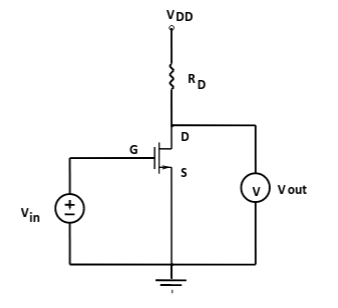
\includegraphics[width=.8\textwidth]{Figures/L5F1}
  \caption{MOSFET Inverter ($R_D=10[\si{\kilo\ohm}]$, $V_{DD}=10[\si{\volt}]$, $0\leq V_{in}\leq 10[\si{\volt}]$)}
  \label{fig:1}
\end{figure}

Using the MOSFET shown in Figure \ref{fig:1} above, we may obtain the following voltage characteristics:

\begin{center}
  \begin{tabular}[H]{|c|c|c|}
    \hline
    $V_{in}[\si{\volt}]$ & $V_{out}[\si{\volt}]$ & $I_D[\si{\milli\ampere}]$\\
    \hline
    0 & 10 & 0\\
    \hline
    1.332 & 9.95 & $5\cdot10^{-3}$\\
    \hline
    1.761 & 9 & .1\\
    \hline
    1.96 & 8 & .2\\
    \hline
    2.111 & 7 & .3\\
    \hline
    2.241 & 6 & .4\\
    \hline
    2.361 & 5 & .5\\
    \hline
    2.471 & 4 & .6\\
    \hline
    2.582 & 3 & .7\\
    \hline
    2.682 & 2 & .8\\
    \hline
    2.791 & 1 & .9\\
    \hline
    3.182 & .5 & .95\\
    \hline
    10 & .2726 & .98274\\
    \hline
  \end{tabular}
\end{center}

To run through and obtain the above values took 5:56.68 for just the voltage values, and 10:06.15 to get all of the values (voltage and drain current).

\subsection{Threshold Voltage}

Based on our table above, we may conclude that the threshold voltage, $V_T$ is approximately $1.278[\si{\volt}]$. The actual voltage is obtained by plotting the square root of the drain current against the threshold voltage to get:

\begin{figure}[H]
  \centering
  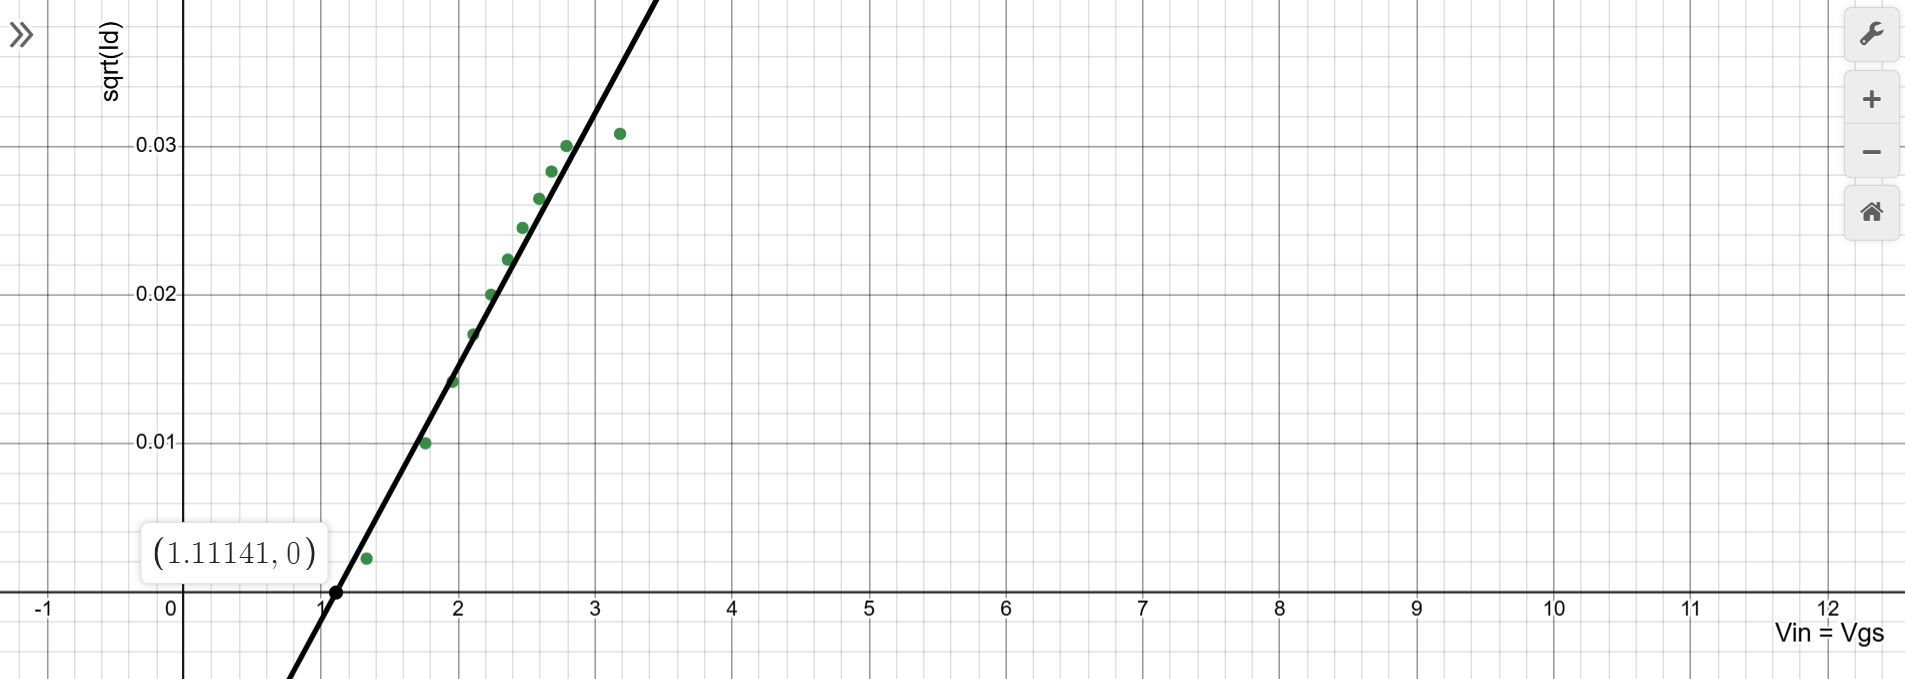
\includegraphics[width=.9\textwidth]{Figures/L5F2}
  \caption{Square Root of Drain Current versus Gate-Source Voltage}
  \label{fig:2}
\end{figure}

From this, we may observe that the threshold voltage is, more accurately, $\boxed{V_T=1.111[\si{\volt}]}$

\subsection{Determining Constant Properties}

We may find the value of:

$$\frac{1}{2}k_n\left( \frac{W}{L} \right)$$

for the MOSFET by simply rearranging our drain current formula to obtain:

$$\frac{1}{2}k_n\left( \frac{W}{L} \right)=\frac{.1}{(1.761-1.278)^2}$$
$$\boxed{\frac{1}{2}k_n\left( \frac{W}{L} \right)=4.287\cdot10^{-3}}$$

\subsection{Transfer Characteristics of the MOSFET}

We may plot the output voltage versus the input to get:

\begin{figure}[H]
  \centering
  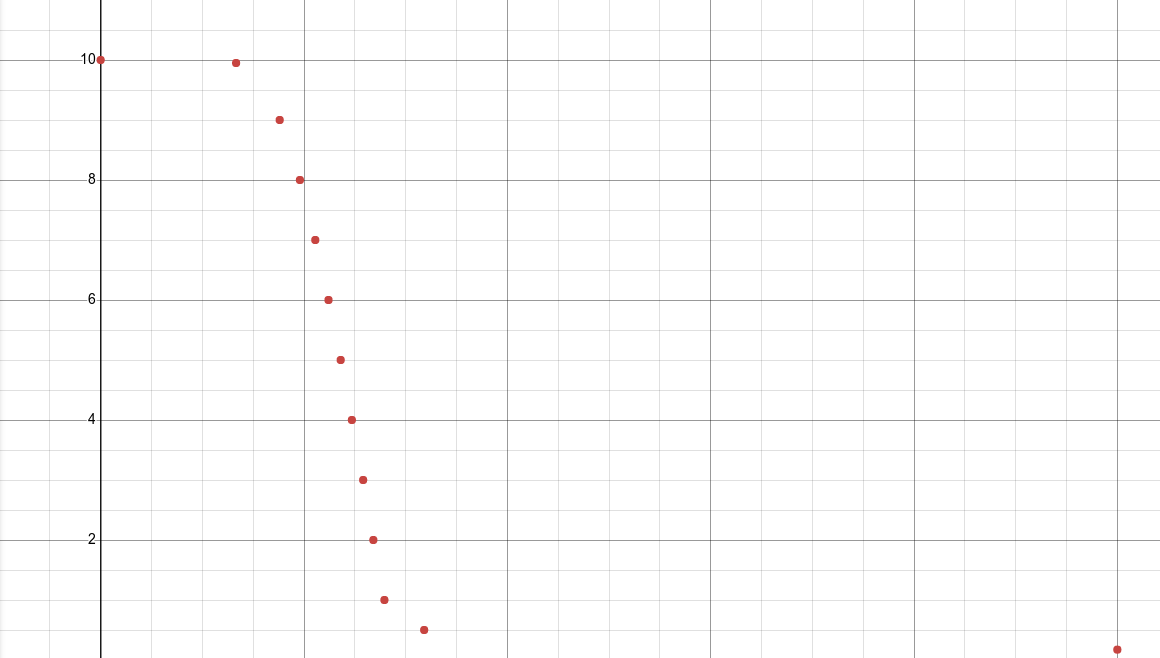
\includegraphics[width=.9\textwidth]{Figures/L5F3}
  \caption{Transfer Characteristic Plot}
  \label{fig:3}
\end{figure}

We may observe from the plot that the modes of operation are, approximately as follows:

$$\boxed{\left\{\begin{array}{ll} \text{Cutoff},&0\leq V_{in}\leq 1.278[\si{\volt}]\\\text{Triode},&1.278\leq V_{in}\leq 3.182[\si{\volt}]\\\text{Saturation},&3.182\leq V_{in}\leq 10[\si{\volt}]\end{array}}$$

\subsection{Calculating the ``On'' Resistance}

We may calculate the ``on'' resistance at the point when $V_{in}=10[\si{\volt}]$. We may write this as:

$$R_{on}=\frac{V_{DS}}{I_D}$$

Since we know $V_{DS}=V_{out}$, we write:

$$R_{on}=\frac{.1726}{.98279\cdot10^{-3}}$$
$$\boxed{R_{on}=175.63[\si{\ohm}]}$$

Since this value is greater than zero, this is not an ideal switch.

\subsection{Determining the Bias Point}

We know that the bias point occurs where the slope of the transfer plot is greatest. We observe that this occurs at $V_{GS}=2.361[\si{\volt}]$ and $V_{DS}=5[\si{\volt}]$. The voltage gain at this point would be (inverted):

$$A_v=-\frac{5}{2.361}$$
$$\boxed{A_v=-2.1177}$$

\subsection{Applying MOSFETs to CMOS Logic}

We may construct the following circuit by using two of the transistors on the CD4007 chip:

\begin{figure}[H]
  \centering
  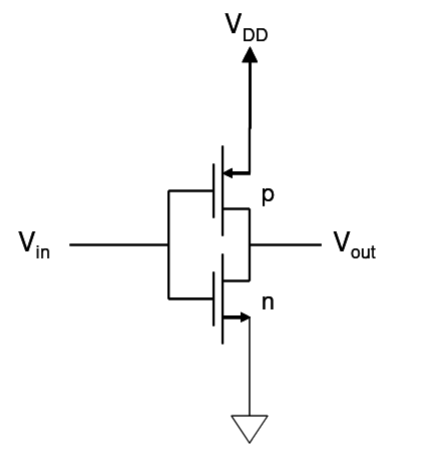
\includegraphics[width=.6\textwidth]{Figures/L5F4}
  \caption{CMOS Logic Inverter}
  \label{fig:4}
\end{figure}

We may use this in a similar manner as the initial circuit, and find the voltage transfer characteristics:

\begin{center}
  \begin{tabular}[H]{|c|c|c|}
    \hline
    $V_{in}[\si{\volt}]$ & $V_{out}[\si{\volt}]$\\
    \hline
    0 & 10\\
    \hline
    1.89 & 9.95\\
    \hline
    3.62 & 9\\
    \hline
    4.28 & 8\\
    \hline
    4.56 & 7\\
    \hline
    4.7 & 6\\
    \hline
    4.77 & 5\\
    \hline
    4.83 & 4\\
    \hline
    4.88 & 3\\
    \hline
    4.98 & 2\\
    \hline
    5.56 & 1\\
    \hline
    6.36 & .5\\
    \hline
    10 & $10[\si{\micro\volt}]$\\
    \hline
  \end{tabular}
\end{center}

\subsection{CMOS Logic Transfer Characteristics}

We then plot this to get:

\begin{figure}[H]
  \centering
  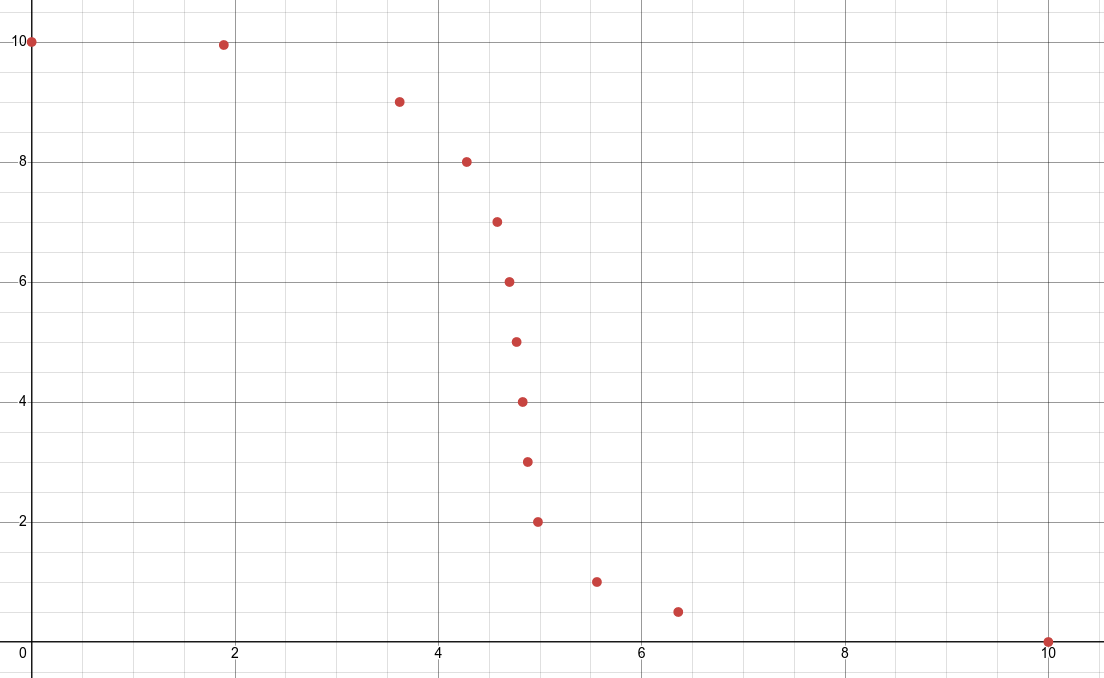
\includegraphics[width=.9\textwidth]{Figures/L5F5}
  \caption{CMOS Logic Inverter Transfer Characteristics}
  \label{fig:5}
\end{figure}

We may determine that the bias point occurs at $(4.77,5)$, which gives us a gain of:

$$A_v=-\frac{5}{4.77}$$
$$\boxed{A_v=-1.0482}$$

We know that there is know power dissipation in a logic circuit.

\subsection{Building a 3-Input NOR Gate}

We construct the following circuit:

\begin{figure}[H]
  \centering
  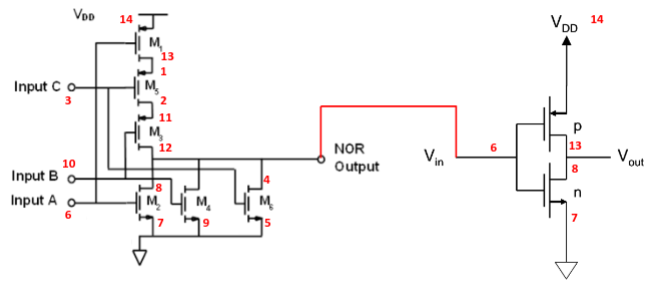
\includegraphics[width=.9\textwidth]{Figures/L5F6}
  \caption{3-Input NOR Gate Using MOSFETS}
  \label{fig:6}
\end{figure}

The physical construction of this looks like:

\begin{figure}[H]
  \centering
  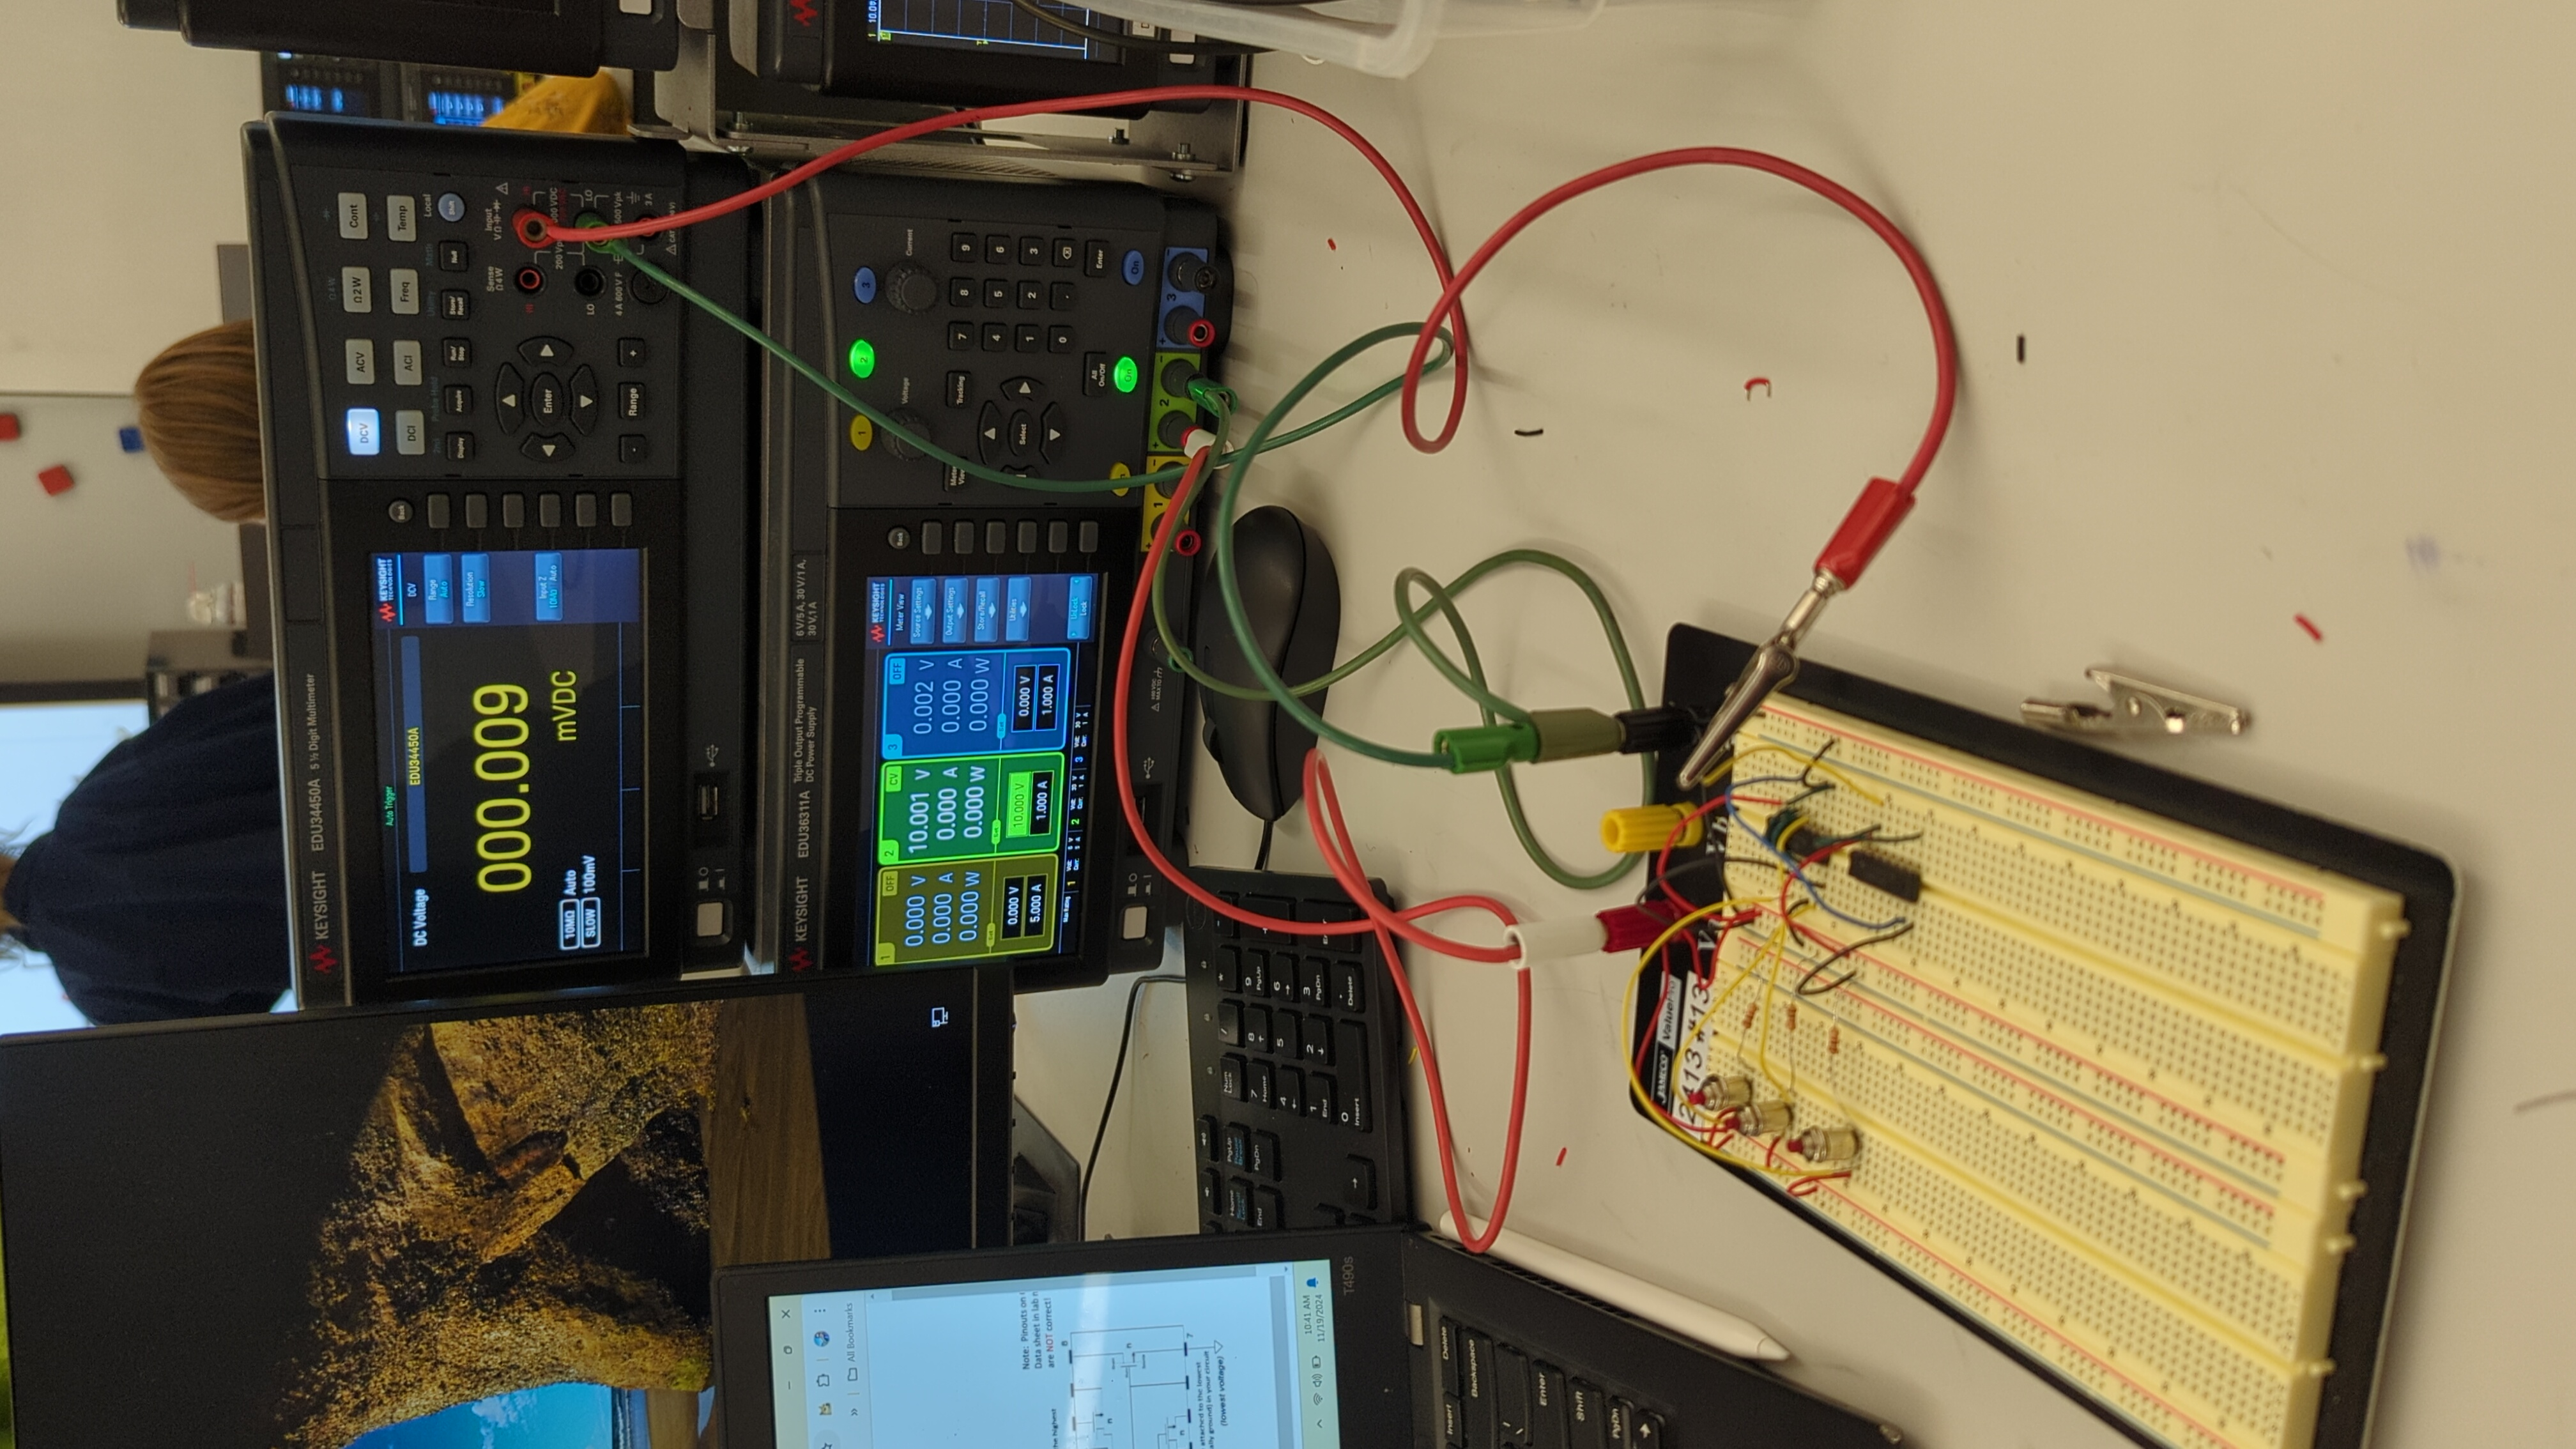
\includegraphics[width=.7\textwidth,angle=270]{Figures/L5F7}
  \caption{Physical 3-Input NOR Gate Circuit}
  \label{fig:7}
\end{figure}

The behavior of the circuit is as expected, and can be seen below:

\begin{figure}[H]
  \centering
  
\includegraphics[width=.4\textwidth]{Figures/L5F8}
  \caption{Scan to View Circuit Behavior}
  \label{fig:8}
\end{figure}

\section{Conclusion}

Overall, this laboratory experiment allowed the performed to get a better understanding of the operation and applications of MOSFETs to various circuitry.

\end{document}
